\chapter{Introduction}
% Argumentation in general and in research.
We all encounter arguments in our lives frequently. When talking to friends, listening to political discussions, or even making decisions in our head. These arguments can get heated and complex since humans have different beliefs and motivations. Finding a common ground or a ''correct`` conclusion is complicated and sometimes impossible. However, these imperfections are what make us humans. \ac{AI}, conversely, needs to act precisely and logically \cite{DBLP:journals/frai/DietzKM24}. To do so, the data needs to be stored and structured in a way, that AI can extract informations from it. This is part of knowledge representation and reasoning and that is why much research is being done in that field \cite{DBLP:journals/dagstuhl-manifestos/DelgrandeG0TW24, DBLP:journals/inffus/PopescuD23}.

% Abstraction of Argumentation -> promises and conclusions, attacks
Arguments can have many forms \cite{Toulmin_2003}. For instance, arguments can be seen as derivations of conclusions, based on assumptions or premises. Such premises can be facts or defeasible assumptions. Relations among arguments are key for driving (automated) argumentative reasoning. A prominent relation between arguments is that of an attack relation, or counter-argument relation. For instance, an argument might attack another. As an example, one argument might conclude that a square is red, while another is concluding that a square is blue. These two arguments are conflicting, and mutually attack each other. Another example would be that an argument is based on a witness statement, while a counter-argument to this one claims that the witness is not truthful, leading to a one-directional attack.



% Abstract Models of argumentation. Graphs.
If an argument $a$ is a counterargument of another argument $b$, we can say that $a$ attacks $b$. With this abstraction, we can abstract our model with directed graphs. The arguments are represented as nodes, and the attacks as directed edges \cite{DUNG1995321}. Now we can define argumentation frameworks (AFs) and use them to evaluate conclusions \cite{DBLP:conf/fapr/Geffner96}. In many cases, viewing arguments as abstract entities is sufficient to carry out argumentative reasoning. Such reasoning is defined via so-called argumentation semantics, which define criteria which (sets of) arguments are deemed jointly acceptable. One of the first pioneers in the topic of argumentation frameworks was Dung. He defined the structure and functionalities in 1995 \cite{Dung1995-DUNOTA-2}.

% Semantics with AFs
% Computation
Semantics define subsets of arguments that have a certain relation to each other. Dung defined different semantics \cite{Dung1995-DUNOTA-2} like conflict-free (cf), admissible (adm) and stable (stb). To be precise, conflict-free and admissible are semantical properties but we will treat them as semantics. According to Dung's definitions, a set \textit{S} is conflict-free if there are no attacks between the arguments in \textit{S}. The definition of conflict-freeness is mainly a building block for the other semantics.
A stable extension, is a conflict-free set, if every argument, which is not in \textit{S}, has an attacker which is in \textit{S}.
Finally, an admissible set is a conflict-free set, where each argument in \textit{S} has a defender in \textit{S}. A defender is this context means an argument which attacks an attacker of an argument in \textit{S}.


% Clustering of AFs
Since AFs can get very big and complicated, another layer of abstraction can be added. This abstraction layer is called \emph{clustering} and generalizes multiple arguments into one bundled cluster \cite{DBLP:conf/kr/SaribaturW21}. In this thesis we refer to the clustered AF as \emph{abstract AF} and the original AF, where no clustering occurs is called \emph{concrete AF}.
Clustering of arguments is a technique to reduce the number of arguments and to provide a high-level view of a given AF. Here, clustering means that arguments can be clustered together in clusters (or clustered arguments). In general, as is the case with many abstraction techniques, clustering can change conclusions that can be drawn from an abstracted formalism. A clustering is said to be \emph{faithful} if no erroneous conclusions can be drawn that is not part of the original, non-abstracted, structure. Otherwise, if conclusions can be drawn that are not there on the original structure, we say that these are \emph{spurious} conclusions.

In our case, the semantics of conflict-free, admissibility, and stable semantics were "lifted`` to the case with clustered arguments. That is, a clustered (abstracted) version of conflict-free sets, admissible sets, and stable extensions was defined on clustered AFs. These semantics respect the clustering of arguments. Then, e.g., an abstract admissible set is spurious if there is no (concrete, non-abstract) admissible set matching this one in the concrete AF. If no such spurious sets exist, then the clustered AF is said to be faithful, w.r.t.\ the concrete AF.






% Example
For instance, let us consider a real-world example like the weather. We can define arguments.

\begin{itemize}
    \item $a$: The sky is blue.
    \item $b$: The atmosphere scatters the sunlights and makes the sky appear blue.
    \item $c$: There exist photographs of a blue sky.
    \item $d$: Photographs can be fake.
    \item $e$: At sunrise the sky appears to be orange.
    \item $f$: Observations can alter, depending on the time.
\end{itemize}

With this knowledge basis, we can create a concrete AF $G=(A, R)$. Where we abstract the arguments into nodes and transform the opposing statement into attacks as shown in \cref{fig:IntroductionComparison}(a). An opposing statement in this context would be for instance the argument $a$ (i.e.\ \emph{The sky is blue}) and $e$ (i.e.\ \emph{At sunrise the sky appears to be orange}). Since both statements can not be true at the same time, they are contradicting, or in other words, attacking each other. If we apply another layer of abstraction, we obtain, e.g.\ the abstract AF $\hat{G}=(\hat{A}, \hat{R})$ defined in \cref{fig:IntroductionComparison}(b). We call arguments which are clustered, \emph{clustered arguments} and arguments which are not in clusters \emph{singletons}. Here, we created a single cluster consisting of the arguments $\{a, b, c, e, f\}$.



\vspace{0.3cm}
\begin{figure}[h]
    \centering
    \begin{subfigure}[t]{0.45\textwidth}
        \centering
        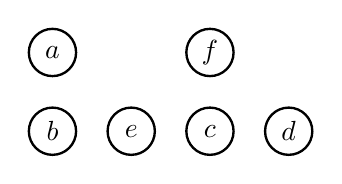
\begin{tikzpicture}
            % Singletons
            \def \ax{0}     \def \ay{0}
            \def \bx{0}     \def \by{-1}
            \def \cx{2}     \def \cy{-1}
            \def \dx{3}     \def \dy{-1}
            \def \ex{1}     \def \ey{-1}
            \def \fx{2}     \def \fy{0}

            \draw[line width=0.3mm] (\ax, \ay) circle (0.3) node[anchor=center]{$a$};
            \draw[line width=0.3mm] (\bx, \by) circle (0.3) node[anchor=center]{$b$};
            \draw[line width=0.3mm] (\cx, \cy) circle (0.3) node[anchor=center]{$c$};
            \draw[line width=0.3mm] (\dx, \dy) circle (0.3) node[anchor=center]{$d$};
            \draw[line width=0.3mm] (\ex, \ey) circle (0.3) node[anchor=center]{$e$};
            \draw[line width=0.3mm] (\fx, \fy) circle (0.3) node[anchor=center]{$f$};

            % Attacks
            \DrawAttackHorizontal{L}{\fx}{\fy}{\ax}{\ay}
            \DrawAttackHorizontal{B}{\ex}{\ey}{\bx}{\by}
            \DrawAttackHorizontal{B}{\cx}{\cy}{\ex}{\ey}
            \DrawAttackHorizontal{L}{\dx}{\dy}{\cx}{\cy}
            \DrawAttackVertical{D}{\fx}{\fy}{\cx}{\cy}
            \DrawAttackDiagonal{PB}{\fx}{\fy}{\ex}{\ey}
            \DrawAttackDiagonal{NB}{\ax}{\ay}{\ex}{\ey}
        \end{tikzpicture}
        \subcaption{Concrete AF $G$}
        \label{af:introExample1}
    \end{subfigure}%
    \begin{subfigure}[t]{0.45\textwidth}
        \centering
        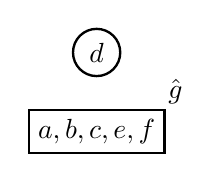
\begin{tikzpicture}
            % Singletons
            \def \gx{0}     \def \gy{-1}
            \def \dx{0}     \def \dy{0}

            \node[rectangle, draw, line width=0.3mm] at (\gx, \gy) {$a,b,c,e,f$};
            \node at (1, -0.5) {$\hat{g}$};
            \draw[line width=0.3mm] (\dx, \dy) circle (0.3) node[anchor=center]{$d$};

            % Attacks
            \DrawSelfAttackLeftTopCluster{\gx-0.8}{\gy + 0.3}
            \DrawAttackVertical{D}{\dx}{\dy}{\gx}{\gy}
        \end{tikzpicture}
        \subcaption{Abstract AF $\hat{G}$}
        \label{af:introExample2}
    \end{subfigure}
    \caption{Concrete and abstract AF}
    \label{fig:IntroductionComparison}
\end{figure}





Now we can compute the sets of the according semantics (cf, adm, stb). The definitions of the semantics are defined in the \cref{ch:Background}. To reduce cluttering, we keep this example to the stable semantics. The stable extensions of the AF $G$ are $stb(G) = \bigl\{\{d, e\}, \{b, d, f\}\bigl\}$.

By computing the stable extensions of the abstract AF $\hat{G}$ $stb(G) = \bigl\{\{d\}, \{d, \hat{g}\}\bigl\}$, we can observe that the AF is spurious due to the extension $\{d\}$, since the abstract stable extension cannot be mapped to one of the concrete stable extensions.

When concretizing (i.e. removing an argument from the cluster) the argument $c$, we create a new AF $\hat{G}' = (\hat{A}', \hat{R}')$ depicted in \cref{af:introExample3}, which has the following stable extensions $stb(G) = \{\hat{g}, d\}$. This extension can be mapped to both stable extensions of the concrete AF $G$, by mutating the cluster $\hat{g}$ with $\{e\}$ or $\{b, f\}$. Thus, we created a faithful abstract AF.

\begin{figure}[h]
    \centering
    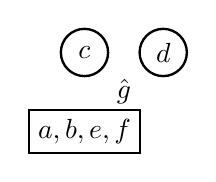
\begin{tikzpicture}
        % Singletons
        \def \gx{0}     \def \gy{-1}
        \def \dx{1}     \def \dy{0}
        \def \cx{0}     \def \cy{0}

        \node[rectangle, draw, line width=0.3mm] at (\gx, \gy) {$a,b,e,f$};
        \node at (0.5, -0.5) {$\hat{g}$};
        \draw[line width=0.3mm] (\dx, \dy) circle (0.3) node[anchor=center]{$d$};
        \draw[line width=0.3mm] (\cx, \cy) circle (0.3) node[anchor=center]{$c$};

        % Attacks
        \DrawSelfAttackLeftTopCluster{\gx-0.65}{\gy + 0.3}
        \DrawAttackHorizontal{L}{\dx}{\dy}{\cx}{\cy}
        \DrawAttackVertical{B}{\cx}{\cy}{\gx}{\gy}
    \end{tikzpicture}
    \caption{Concretized AF $\hat{G}'$}
    \label{af:introExample3}
\end{figure}


% Importance of concretizing single arguments
When producing an AF with multiple layer of abstractions, we obtain a high-level view of the concrete AF. This simplification has the drawback to lose some details. To still have a deep understanding of the structure to some extend, extracting single arguments of the cluster by concretizing them can be helpful. This also allows the user to have a direct impact to the outcome and produce customized faithful AFs.


% What we want to show in this paper
% Main contributions in this paper
%Complexity
Creating abstract, faithful AFs can be challenging and is the main focus of this thesis. Unfortunately, drawing a conclusion from an AF can be challenging, e.g., it can be NP-complete and sometimes even be beyond NP to decide whether an argument is acceptable under a specific argumentation semantics \cite{DBLP:journals/ai/DvorakGRW23}. In fact, the complexity of proving faithfulness or spuriousness of an AF is $\prod_2^P$ hard \cite{DBLP:conf/kr/SaribaturW21}. In practice, this means, that to obtain a result, multiple instances or calls of a SAT-Solver need to be invoked.

We created one of the first tools to produce an abstract AFs based on a concrete AFs. We cover different setups and usages, including different semantics and base functionalities. The main contributions of this thesis are as follows.

\begin{itemize}
    \item We provide algorithms for computing abstract semantics of a given clustered AF. That is, our algorithms are capable of computing or enumerating all extensions under abstract conflict-free, admissible, and stable semantics.

    \item Based on our algorithms for computing abstract semantics, we provide algorithmic solutions for checking faithfulness of a given clustered AF. We develop two approaches in this regard: (i) one of based on breadth-first-search (BFS) and (ii) one based on depth-first search (DFS). While the algorithm based on BFS first calculates all original extensions and abstract extensions of a given AF and clustered AF, respectively, the DFS variant iteratively computes abstract extensions of the clustered AF and verifies (non-)spuriousness of this extension.

    \item Towards user-interaction, for a given AF and clustered AF, we provide an algorithm for concretization, by which we mean that a user can select arguments inside clusters to be made concrete (singletons). We then refine the clustered AF until faithfulness is reached, since the extraction of the user-defined arguments may result in spurious reasoning.
    
    \item We implemented our algorithms in TODO how? and provide the implementations in open-source.
    \item In an experimental evaluation, $\cdots$ TODO results.
    \item $\cdots$
\end{itemize}

We provide an open source implementation of the previously listed tools \cite{Pasero2024-AFClustering-Repo}.

\begin{center}
    \url{https://github.com/p4s3r0/argumentation-framework-clustering}
\end{center}

\noindent

\textit{TODO: Further contributions}

\textit{TODO: Choice of methods to obtain results}

\textit{TODO: How big AFs are still feasible to solve}
